\documentclass[11pt,a4paper]{article}
\usepackage[T1]{fontenc}
\usepackage[utf8]{inputenc}
\usepackage{lmodern,microtype}
\usepackage[margin=22mm,headheight=15pt]{geometry}
\usepackage{amsmath,amssymb,booktabs,tabularx,array,enumitem}
\usepackage{xcolor,graphicx}
\usepackage{tikz}
\usetikzlibrary{arrows.meta,positioning,shapes.geometric}
\usepackage{tcolorbox}
\tcbuselibrary{breakable}
\usepackage{fancyhdr,hyperref}
\definecolor{ink}{HTML}{18354A}
\definecolor{teal}{HTML}{087E8B}
\definecolor{pale}{HTML}{EDF5F6}
\definecolor{gold}{HTML}{AD6B20}
\hypersetup{colorlinks=true,linkcolor=teal,citecolor=teal,urlcolor=teal,pdftitle={Constructing an Agent-Based Model},pdfauthor={ABM course}}
\pagestyle{fancy}\fancyhf{}
\fancyhead[L]{\small\sffamily ABM\_course\quad /\quad Session 4}
\fancyhead[R]{\small\sffamily Construction and ontology}
\fancyfoot[L]{\footnotesize\sffamily Constructing an Agent-Based Model}
\fancyfoot[R]{\sffamily\thepage}
\renewcommand{\headrulewidth}{0.3pt}
\setlength{\emergencystretch}{2em}
\setlength{\parindent}{0pt}\setlength{\parskip}{6pt}
\setcounter{secnumdepth}{3}
\setcounter{tocdepth}{2}
\raggedbottom
\setlist{nosep,leftmargin=1.5em}
\newtcolorbox{principle}[1]{breakable,colback=pale,colframe=teal,boxrule=.6pt,arc=2pt,title={#1},fonttitle=\bfseries,top=5pt,bottom=5pt}
\newcommand{\stereo}[1]{\texttt{\guillemotleft #1\guillemotright}}
\newcommand{\stage}[1]{\textsf{\textbf{#1}}}
\newcolumntype{P}[1]{>{\raggedright\arraybackslash}p{#1}}
\newcolumntype{Y}{>{\raggedright\arraybackslash}X}
\tikzset{box/.style={draw=teal,fill=pale,rounded corners=2pt,align=center,font=\small,inner sep=7pt},arr/.style={-{Stealth[length=2mm]},thick,draw=ink}}

% Fit long display equations to the available width without altering their content.
\newsavebox{\displaybox}
\newenvironment{fitdisplay}{\par\medskip\noindent\begin{lrbox}{\displaybox}$\displaystyle}{% 
$\end{lrbox}\makebox[\linewidth][c]{\ifdim\wd\displaybox>\linewidth\resizebox{\linewidth}{!}{\usebox{\displaybox}}\else\usebox{\displaybox}\fi}\par\medskip}
\begin{document}
\thispagestyle{empty}
{\sffamily\color{teal}\large ABM\_course / Teaching guide / Session 4\par}
\vspace{7mm}
{\sffamily\bfseries\color{ink}\fontsize{28}{32}\selectfont Constructing an\\Agent-Based Model\par}
\vspace{4mm}
{\large From Organized Complexity to Prospective Claims and Actionability\par}
\vspace{5mm}

\section*{Purpose}

The central methodological problem is not simply how to program an ABM. It is:

\begin{fitdisplay}
\boxed{\textbf{How do we decide what ABM to construct?}}
\end{fitdisplay}

Once the model exists, a second problem follows:

\begin{fitdisplay}
\boxed{\textbf{What can we defensibly claim from it?}}
\end{fitdisplay}

The guide therefore moves from \textbf{ex-ante construction} to \textbf{ex-post accountability}:

\begin{fitdisplay}
\boxed{
\text{EX ANTE: CONSTRUCT}
\rightarrow
\text{SIMULATE}
\rightarrow
\text{EX POST: DOCUMENT \& ASSESS}
}
\end{fitdisplay}



\clearpage
\begin{principle}{Source boundaries and course terminology}
This session introduces six new readings that build on the foundations developed in earlier sessions, including Simon \cite{simon_behavioral_1955,simon}, Weaver \cite{weaver}, Axtell \cite{axtell_why_2000-1}, Macy--Willer \cite{macy_factors_2002}, and Kollman--Page \cite{kollman_chapter_2006}. The guide brings those earlier foundations into conversation with the new readings to address ABM construction. Citations distinguish reading-grounded contributions from this course's synthesis. ``Bottom-up + along the way,'' the Four As, the parsimonious I-ABM heuristic and the distinction between $A_{3m}$ and $A_{3s}$, auditability/actionability, and the broad use of ``meta-analysis'' are course conventions. The six-class relational grammar, situated-agency triad, and practice-transition notation introduced below are also course synthesis. They are not attributed as a combined framework to the readings.

Ex ante and ex post distinguish methodological questions. Documentation can begin during construction, and later assessment can prompt revision.
\end{principle}
\clearpage
\tableofcontents
\clearpage
\section{From Previous Sessions: Foundations for Studying Complex Systems}
\label{sec:previous-foundations}

Session 4 builds on the earlier readings. Their contributions establish why organization, agency, and interaction matter, and why agent-based computation can be useful for studying them.

\begin{description}[style=nextline,leftmargin=0pt,labelindent=0pt,labelsep=0pt,labelwidth=0pt,itemindent=0pt,itemsep=6pt]
\item[Weaver --- Organized complexity]
Weaver distinguishes simplicity, disorganized complexity, and organized complexity. The latter directs attention to interdependent factors whose organization matters to the phenomenon \cite{weaver}.

\item[Simon --- Decision-making and the architecture of complexity]
Simon's behavioral account of rational choice brings information and computational limits into the representation of decision-making \cite{simon_behavioral_1955}. His account of hierarchy and near-decomposability highlights subsystems and the differences between interactions within and between them \cite{simon}. Together, these readings draw attention to both decision processes and system organization.

\item[Axtell --- Why use agents?]
Axtell distinguishes uses of agent computation according to its relationship with mathematical formulations: presenting or computing solutions, exploring models that cannot be fully solved, and systematically investigating processes for which an equation-based formulation is not useful \cite{axtell_why_2000-1}. The reason for choosing ABM therefore depends on the problem being investigated.

\item[Macy--Willer --- From factors to actors]
Macy and Willer examine social processes through interacting adaptive agents and show how local interactions can generate aggregate patterns. Their review emphasizes relational microfoundations, networks that shape and are shaped by interaction, and computational experiments \cite{macy_factors_2002}.

\item[Kollman--Page --- Computational models of politics]
Kollman and Page connect computational modeling to political questions, including collective action, institutional design and performance, and electoral competition. Their discussion highlights adaptation, differences among agents, externalities, path dependence, geography, networks, and emergence \cite{kollman_chapter_2006}.
\end{description}

\begin{principle}{The transition to Session 4}
These earlier contributions motivate attention to organized complexity, bounded decision-making, interaction, and computational inquiry. The course now turns to a construction question: \textbf{How do we decide what ABM to build?} The following heuristics organize our response; they are course synthesis rather than a shared framework proposed by the earlier authors.
\end{principle}

\clearpage
\section{Foundations: Thinking About ABM Construction}

Building on those earlier foundations, two heuristics organize ABM construction in Session 4:

\begin{fitdisplay}
\boxed{\textbf{BOTTOM-UP}}
\qquad+\qquad
\boxed{\textbf{ALONG THE WAY}}
\end{fitdisplay}

These are \textbf{not opposites}.

\begin{itemize}
\item \textbf{Bottom-up} organizes a generative spiral of model construction and revision.
\item \textbf{Along the way} identifies additional questions that arise as the model is progressively constructed.
\end{itemize}

\subsection{Bottom-Up: The Generative Spiral}

The \textbf{generative spiral} is a course synthesis drawing on three contributions: Epstein supplies the generative question; Axelrod emphasizes simplicity and simulation as an aid to intuition; and Cioffi-Revilla supplies progressive model construction inspired by Lakatos \cite{epstein,axelrod_complexity_1997,cioffi}. Together, these contributions guide what we seek to generate, how we keep its mechanisms understandable, and how we revise the specification. Progress need not mean adding detail.

\subsubsection{Epstein --- Generate}

Epstein asks how a micro-specification can generate a macro-regularity \cite[pp.~41--43]{epstein}. Generation provides a candidate explanation; it does not uniquely identify the real mechanism. The generative question is:

\begin{quote}
\textbf{How could local interactions among heterogeneous autonomous agents generate the macro-pattern of interest?}
\end{quote}

\begin{fitdisplay}
\boxed{
\text{Micro-specification}
\rightarrow
\text{Interaction}
\rightarrow
\text{Macro-pattern}
}
\end{fitdisplay}

The modeller constructs the model, not its emergent outcome:

\begin{fitdisplay}
\boxed{
\text{CONSTRUCT THE MODEL}
\neq
\text{CONSTRUCT THE OUTCOME}
}
\end{fitdisplay}

Therefore:

\begin{fitdisplay}
\boxed{\textbf{Construct the conditions of possibility, not the emergent result.}}
\end{fitdisplay}

\subsubsection{Axelrod --- Keep It Simple and Aid Intuition}
\label{sec:axelrod-foundation}

Axelrod presents agent-based modeling as a way to aid intuition and advocates \textbf{KISS}: ``keep it simple, stupid'' \cite[pp.~4--6]{axelrod_complexity_1997}. Begin with assumptions simple enough that we can understand how the specified interactions produce the observed results. Complexity in the outcome need not require complexity in every assumption.

Simulation can also challenge intuition. Axelrod's cultural-dissemination model shows how a simple mechanism can produce results that prompt us to reconsider expectations and formulate new questions \cite[pp.~219--220]{axelrod_dissemination_1997}. A model that aids intuition may therefore yield counterintuitive results.

\begin{quote}
\textbf{What can a deliberately simple model teach us, and can we trace how its mechanisms produce that result?}
\end{quote}

In our construction heuristic, this principle applies throughout revision: justify each additional distinction by what it contributes to the question. Simplicity concerns the whole model, including agents, environments, decision processes, and connections. The later I-ABM discussion expresses this principle through the course's Four As.

\subsubsection{Cioffi-Revilla --- Construct Progressively}

Cioffi-Revilla motivates theoretically guided model sequences with inspiration from Lakatos \cite{cioffi}. The course develops this into explicit ontological re-specification, including removal and reclassification. Begin with a deliberately restricted model and progressively re-specify it:

\begin{fitdisplay}
\boxed{
O_0\rightarrow O_1\rightarrow O_2\rightarrow\cdots
}
\end{fitdisplay}

Progressive construction is \textbf{not}:

\begin{fitdisplay}
O_{n+1}=O_n+\text{more detail}
\end{fitdisplay}

Instead:

\begin{fitdisplay}
\boxed{
O_{n+1}=\operatorname{re-specify}(O_n)
}
\end{fitdisplay}

using operations such as:

\begin{fitdisplay}
\boxed{
\text{ADD}
\quad
\text{REMOVE}
\quad
\text{DE-/RECLASSIFY}
\quad
\text{RECOMBINE}
}
\end{fitdisplay}

These operations have the following meanings in the course's construction vocabulary:

\begin{description}[style=nextline,leftmargin=0pt,labelindent=0pt,labelsep=0pt,labelwidth=0pt,itemindent=0pt,itemsep=4pt]
\item[ADD] Introduce an element, attribute, capability, or relation previously absent from the specification because the question now requires it.
\item[REMOVE] Eliminate a represented element or distinction that is unnecessary, redundant, or no longer justified for the question.
\item[DE-/RECLASSIFY] Revise existing categories or modeling roles---for example, split one category into two, merge two categories, or change an element from one type to another.
\item[RECOMBINE] Reorganize how represented elements are connected or grouped, changing the configuration of the system.
\end{description}

A revision may combine several operations; each should be justified by the modeling question.

Thus:

\begin{fitdisplay}
\boxed{
\textbf{Progressive construction}
=
\textbf{progressive ontological re-specification}
}
\end{fitdisplay}



\subsection{Along the Way: Balancing Parsimony and Context}

Parsimony keeps representation focused on the modeling question. Along the way, contextual requirements can reveal which initial simplifications need revision. We consider institutional structuring through Ghorbani/Ostrom, situated agency through Knoeri/Giddens, and then social recursivity. These complementary contributions help us reconsider what is minimally sufficient for the question.

\subsubsection{Ghorbani / Ostrom --- Institutionally Structured Agency}

When institutional prescriptions matter to the question, the usefulness of the model depends on representing their actual role in action. Listing the rules is insufficient: we need to specify how agents respond to them. Ask:

\begin{quote}
\textbf{How do institutional prescriptions influence what agents actually do?}
\end{quote}

Institutions structure action possibilities without mechanically determining behavior:

\begin{fitdisplay}
\boxed{
\text{Institution}
\rightarrow
\text{Structured possibilities}
\rightarrow
\text{Agent decision}
\rightarrow
\text{Action}
}
\end{fitdisplay}

Ghorbani et al., building on Ostrom's institutional analysis, discuss how institutions structure action and how agents respond to institutional prescriptions \cite{ghorbani}. We draw on this contribution to examine institutions and their enactment: what is prescribed and what agents actually do. \footnote{MAIA (Modelling Agent systems based on Institutional Analysis) is Ghorbani et al.'s framework, developed from Ostrom's IAD (Institutional Analysis and Development). They provide the background to the reading's treatment of institutions \cite{ghorbani}.}

\begin{principle}{From institutional prescriptions to rules in use}
Ostrom's emphasis on the rules actually used to organize recurring interaction, as presented by Ghorbani et al., directs attention to how institutions operate in practice \cite[sec.~2.3]{ghorbani}. Identifying a prescription is therefore a starting point: how does it enter agents' decisions and the interactions that follow?

Ghorbani et al. explicitly allow agents to disregard institutions under certain conditions \cite[sec.~2.4]{ghorbani}. An obligation specifies what an agent should do; it does not guarantee compliance. If compliance varies in reality, making every agent follow every prescription removes a potentially important source of variation and limits the model's ability to explain how institutions operate in practice.
\end{principle}

The modeling task is therefore to represent how agents respond to prescriptions. Their commitment to institutional goals, immediate needs, and expected sanctions may influence compliance; which factors to include depends on the question.

For example, agents asked to limit their use of a shared resource may comply out of commitment to conservation or fear of sanctions, while others exceed the limit to meet immediate needs. This course illustration shows why prescribing a limit and modeling its effects are different tasks.

As agents encounter institutions---through acceptance, habit, or coercion---their expectations and ways of acting may change. How can we represent agents whose decisions are shaped by these conditions, and whose actions may, in turn, reproduce or transform them?

\subsubsection{Knoeri / Giddens --- Situate Agency}

\begin{fitdisplay}
\boxed{\textbf{Agency is situated.}}
\end{fitdisplay}

The parsimony maintained so far may now require a substantial revision: the question may demand agents whose decisions are sensitive to their context. Knoeri et al. provide an approach to operationalizing context-specific agents, interactions, decisions, and behavior, drawing on Giddens and empirical knowledge of the system \cite{knoeri}.

Context extends beyond other agents. It includes the environment in which action occurs and the artifacts and institutional conditions that enable, constrain, or mediate it. In the course vocabulary, we distinguish two forms of \textbf{Artificiality}:

\begin{description}[style=nextline,leftmargin=0pt,labelindent=0pt,labelsep=0pt,labelwidth=0pt,itemindent=0pt,itemsep=4pt]
\item[Material Artificiality] Tools, technologies, infrastructure, and other artifacts that shape what agents can do.
\item[Social Artificiality] Rules, norms, roles, and authority arrangements that shape what agents are expected, permitted, or forbidden to do.
\end{description}

Representing these conditions is only part of the task. We also need to specify how agents perceive and respond to them. A situated agent's decisions depend on its access to material means and its interpretation of social expectations, alongside its own needs and capabilities.

The further construction challenge is to represent agents \textbf{dynamically endogenizing the influence of Artificiality}: experience with tools, rules, and institutions may enter their evolving expectations, habits, and decision processes. For example, repeated use of a tool may change how an agent performs a task; experience with a rule may change its willingness to comply. These are course illustrations of mechanisms to specify when the question requires them, rather than automatic consequences of adding context to the model.

This leads to a further question: how do agents' actions, in turn, reproduce or transform the material and social conditions of subsequent action?

\subsubsection{Giddens --- Social Recursivity}

Through Knoeri et al.'s use of Giddens, we encounter a further idea: agents draw on existing rules and resources when they act, and their practices help reproduce or transform those same conditions \cite{knoeri}. Social structure is therefore both a condition of action and something sustained or changed through action. This is the sense of \textbf{social recursivity} developed here.

\begin{principle}{Recursivity through practice}
People act under conditions inherited from earlier interactions. In using, interpreting, following, or contesting those conditions, they contribute to the conditions of subsequent action. Repetition may sustain an established practice; it may also modify that practice, deliberately or unintentionally.
\end{principle}

A mathematical comparison helps clarify the idea. In the Fibonacci recurrence,
\begin{fitdisplay}
F_{n+1}=F_n+F_{n-1},\qquad F_0=0,\quad F_1=1,
\end{fitdisplay}
the rule and initial values determine each subsequent value. The numbers do not interpret or contest the rule. Social recursivity is less straightforward: people interpret expectations, respond to others, and act with unequal resources and authority. Their actions may sustain or alter the rules and relations organizing their interaction. The comparison is a course illustration, not a claim that Giddens proposes a mathematical recurrence.

For example, people joining a queue encounter an expectation about whose turn comes next. By waiting and recognizing others' turns, they help sustain that convention. If some claim priority and others accept or challenge the claim, the practice may be reinforced, modified, or disputed. The conditions of the next interaction depend partly on what people have just done.

\begin{center}
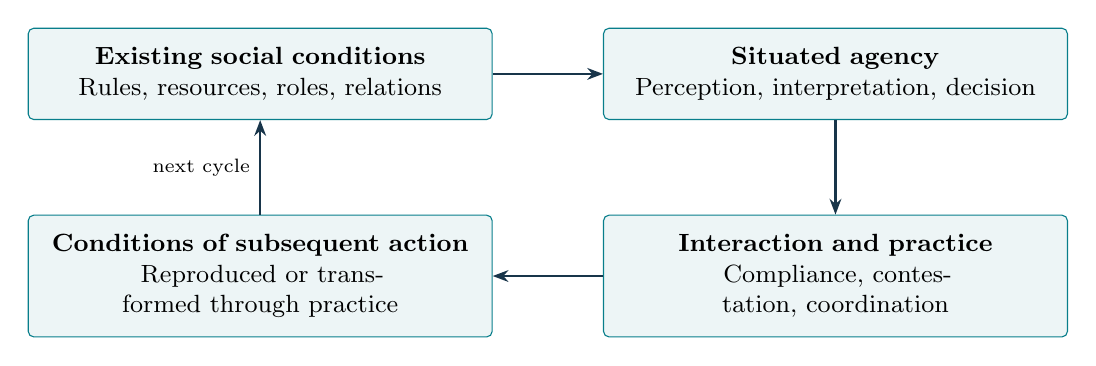
\begin{tikzpicture}[node distance=12mm and 14mm]
\node[box,text width=5.4cm] (s) {\textbf{Existing social conditions}\\Rules, resources, roles, relations};
\node[box,text width=5.4cm,right=of s] (a) {\textbf{Situated agency}\\Perception, interpretation, decision};
\node[box,text width=5.4cm,below=of a] (i) {\textbf{Interaction and practice}\\Compliance, contestation, coordination};
\node[box,text width=5.4cm,below=of s] (n) {\textbf{Conditions of subsequent action}\\Reproduced or transformed through practice};
\draw[arr] (s)--(a);\draw[arr] (a)--(i);\draw[arr] (i)--(n);
\draw[arr] (n)--node[left,font=\scriptsize,align=right]{next cycle}(s);
\end{tikzpicture}
\end{center}
{\small\textbf{Figure 1. Social recursivity through practice (course synthesis).} Arrows show conditioning and the continuation of practice. The next cycle begins under the resulting conditions, which may persist or change. The diagram separates moments for explanation; in social life, these processes may overlap.}

Recursivity does not require constant change: maintaining a convention also depends on its continued enactment. Nor does recursivity alone establish chaos or unpredictability. An ABM can represent these processes with explicitly specified mechanisms, including deterministic ones; the modeling task is to decide how agents' actions sustain or alter the conditions relevant to the question.

A useful \textbf{course synthesis, not a direct quotation}, is:
\begin{fitdisplay}
\boxed{\textbf{History conditions action; practice sustains or transforms its conditions.}}
\end{fitdisplay}

This also provides a course bridge to Simon: organization helps us understand persistence, while Giddens directs attention to the practices through which social organization is reproduced or transformed.

\subsection{Bottom-Up + Along the Way}

The generative spiral proceeds through successive model specifications:

\begin{fitdisplay}
\boxed{
O_0
\longrightarrow
O_1
\longrightarrow
O_2
\longrightarrow
O_n
}
\end{fitdisplay}

But along that trajectory:

\begin{fitdisplay}
\boxed{
\begin{array}{ccccccc}
O_0 &\longrightarrow& O_1 &\longrightarrow& O_2 &\longrightarrow& O_n\\
&&\uparrow&&\uparrow&&\uparrow\\
&&\text{articulate}&&\text{situate}&&\text{empirically}\\
&&\text{institutions}&&\text{agency}&&\text{ground}
\end{array}}
\end{fitdisplay}

The heuristic is:

\begin{fitdisplay}
\boxed{\begin{gathered}
\textbf{Start generatively. Construct progressively.}\\
\textbf{Along the way, situate the model where the question requires it.}
\end{gathered}}
\end{fitdisplay}

These interventions can recur at any revision; they are not compulsory stages. A richer model can remain generative.



\clearpage
\section{Ex Ante: Constructing the Ontology}

The ex-ante question is:

\begin{fitdisplay}
\boxed{\textbf{What are we going to model?}}
\end{fitdisplay}

The construction heuristic is:

\begin{fitdisplay}
\boxed{
\textbf{DISSECT}
\rightarrow
\textbf{DISCRETIZE}
\rightarrow
\textbf{COMBINE}
}
\end{fitdisplay}



\subsection{Dissect}

Start from the phenomenon:

\begin{fitdisplay}
\text{Phenomenon}
\xrightarrow{\text{dissect}}
\text{Relevant distinctions}
\end{fitdisplay}

\textbf{Question:}

\begin{quote}
What distinctions are necessary for investigating the phenomenon?
\end{quote}

Dissection is analytical.



\subsection{Discretize}

Decide which distinctions become explicit modeled elements.

The first three As provide the basic vocabulary:

\begin{fitdisplay}
\boxed{A_1,\;A_2,\;A_3}
\end{fitdisplay}

\subsubsection{\texorpdfstring{\(A_1\)}{A1} --- Agent}

\begin{quote}
\textbf{An entity whose endogenous agency is necessary for the explanatory or decision problem.}
\end{quote}

\textbf{Question:}

\begin{fitdisplay}
\boxed{\text{Who has endogenous agency?}}
\end{fitdisplay}

\subsubsection{\texorpdfstring{\(A_2\)}{A2} --- Arena}

\begin{quote}
\textbf{The material, spatial, ecological, or environmental substrate within which action occurs.}
\end{quote}

\textbf{Question:}

\begin{fitdisplay}
\boxed{\text{Where does action occur?}}
\end{fitdisplay}

\subsubsection{\texorpdfstring{\(A_3\)}{A3} --- Artificiality}

\begin{quote}
\textbf{Human-made artifacts and socially constructed institutions that mediate agents' relations with other elements of the modeled world.}
\end{quote}

Here, \textbf{artificial} means made or instituted through human activity rather than naturally occurring. It does not mean unreal: tools, infrastructure, rules, and institutions can have real effects on action. Artificiality enables, constrains, or redirects how agents interact with one another and with their environment.

\begin{fitdisplay}
\boxed{A_3=A_{3m}+A_{3s}}
\end{fitdisplay}
The plus sign denotes conceptual composition, not numerical addition.

\begin{description}[style=nextline,leftmargin=0pt,labelindent=0pt,labelsep=0pt,labelwidth=0pt,itemindent=0pt]
\item[$A_{3m}$ --- Material Artificiality] Tools, technologies, infrastructure, and other human-made artifacts that mediate action. A traffic-light device can be represented here.
\item[$A_{3s}$ --- Social Artificiality] Institutions, norms, formal rules, roles, and authority arrangements. The obligation to stop at a red light and the authority to sanction violations can be represented here.
\end{description}

Including particular artifacts and institutions makes the model more contextualized: its account of action now depends on those arrangements. This narrows the conditions under which its results can be generalized without further justification. The added specificity should serve the modeling question.

\begin{principle}{Artificiality is not decorative}
Explicit Artificiality adds modeling complexity: its relevant properties, relations, and effects on action must be specified. Represent a traffic light when the intention is to investigate how it affects traffic. This requires specifying what agents perceive and how they respond to its signals, including compliance or non-compliance where relevant. Merely drawing a traffic light does not represent its mediation of action.
\end{principle}

%

A useful heuristic is:
\begin{fitdisplay}
\boxed{\text{Artificiality}=\text{affordance and/or barrier}}
\end{fitdisplay}

\subsection{Combine: \texorpdfstring{\(A_4\)}{A4} --- Array}

Discrete elements must be arranged into a system.

\begin{quote}
\textbf{Array is the assumed systemic arrangement organizing Agents, Arena and Artificiality.}
\end{quote}

\begin{fitdisplay}
\boxed{
A_4=\mathcal C(A_1,A_2,A_3)
}
\end{fitdisplay}

Here, $\mathcal C$ denotes configuration, not a transition rule. At a given time, $A_4(t)=\mathcal C(A_1(t),A_2(t),A_3(t))$ describes the arrangement then obtaining. A configuration can change during a run; the mechanism producing that change is specified separately in dynamics.

\textbf{COMBINE is an explicit modeling operation.} Listing elements and their capabilities does not yet connect them. COMBINE establishes the potential pathways through which methods can affect states of connected elements. A link need not be labeled: it provides a pathway, while each method specifies how it uses that pathway, under which conditions, and which states it may affect. A connection alone produces no effect. The following construction checks make that task concrete:

\begin{description}[style=nextline,leftmargin=0pt,labelindent=0pt,labelsep=0pt,labelwidth=0pt,itemindent=0pt,itemsep=5pt]
\item[Provide a path for influence.] Without a represented path of influence, an element cannot affect or be affected by another. The path may be direct or mediated by other agents, artifacts, or the environment. An indirect connection through the environment must also be specified: one element's method changes an environmental state that another element's method can read or respond to. Mere co-location does not establish influence.

\item[Connect capabilities to their conditions of use.] A method may be correctly specified yet never be enacted because the agent lacks access to the information, resource, or counterpart it requires. A weak or unreliable connection may limit its enactment. For example, if the model includes drivers and traffic lights, a driver's method ``see the color'' requires a connection to the traffic light whose state it reads. The connection provides the pathway; the method specifies how the driver reads the color and under which conditions.

\item[Distinguish connectivity from the direction of effects.] An unlabeled link does not imply mutual effects. The methods using the pathway specify the direction of each effect and whether influence occurs both ways. A driver's perception method may read a signal's state without changing it; a sensor-controlled signal may also use information about approaching vehicles. Neither effect nor reciprocity follows from the line alone.

\item[Exclude genuine isolates.] An element may affect others without itself being affected. Its states may remain fixed, but a connection is still required for another element's method to read or use them. For example, an arena's fixed dimensions may constrain agents' movement. Immutability alone therefore does not make an element decorative. A genuine isolate has no actual or possible connection through which it affects or is affected by the modeled system. Such an element contributes nothing to the modeled interactions: specify the missing connection or remove the unnecessary element.
\end{description}

\begin{principle}{The modeler's judgment becomes especially visible in COMBINE}
Recognizing relevant elements is only part of understanding a system. Deciding how they depend on and influence one another tests the modeler's experience and knowledge of the phenomenon. A plausible inventory can still produce a poorly specified model if essential pathways are missing or methods use them inappropriately. Each connection should be justified by the modeling question, and its uses made explicit in the relevant methods. A label on the line is optional.
\end{principle}

\textbf{Six relational classes.} The following course grammar identifies the kinds of relations to consider, without requiring every class in every model:

\begin{center}
\renewcommand{\arraystretch}{1.2}
\begin{tabularx}{\linewidth}{@{}P{1.7cm}P{4cm}Y@{}}
\toprule
\textbf{Relation} & \textbf{Meaning} & \textbf{Example across models}\\
\midrule
$A_1-A_1$ & Agent relations & Traffic: driver--pedestrian, providing a pathway for each to perceive the other.\\
$A_2-A_2$ & Arena relations & Hydrology: river--soil, providing a pathway for river conditions to affect soil and soil conditions to affect the river.\\
$A_3-A_3$ & Artificiality relations & Traffic: sensor--signal controller, providing a pathway for sensor readings to affect signal timing.\\
$A_1-A_2$ & Agent location & Evacuation: person--room, locating the person within the represented space.\\
$A_1-A_3$ & Institutionally structured agency & Resource use: fisher--fishing quota, providing a pathway for the fisher's decision method to consider the prescribed catch limit.\\
$A_3-A_2$ & Context of Artificiality & Agriculture: irrigation device--soil, connecting the device to the area where its operation can change soil moisture.\\
\bottomrule
\end{tabularx}
\end{center}

These examples illustrate modeling roles: river and soil are Arena in the hydrology example; the sensor and signal controller are material Artificiality in the traffic example. Each connection provides a potential pathway. Methods specify whether and how it is used, including whether effects occur in one or both directions.

The dashes identify relational classes, not mandatory link labels or temporal arrows. These classes help check which kinds of elements are connected. Methods specify the uses, conditions, and direction of effects supported by those connections. This is a \textbf{relational grammar}, not a claim that the system is reducible to a union of dyads. It can express networks, topology, hierarchy, spatial configurations, dependencies, and institutional configurations. Specify the methods that use the connections and any joint conditions needed by the question.

\textbf{Situated agency.} A particularly important triadic configuration is:
\begin{fitdisplay}
\boxed{A_1-A_3-A_2=\text{situated agency}}
\end{fitdisplay}
The triad relates agents to Artificiality within an Arena. Its meaning depends on that joint configuration, not merely on three independent links. In particular:
\begin{fitdisplay}
\boxed{\underbrace{A_1-A_2}_{\text{agent location}}
\neq \underbrace{A_1-A_3-A_2}_{\text{situated agency}}}
\end{fitdisplay}
Locating an agent does not yet specify the institutional and material conditions of its agency. Conversely, situatedness does not require representing every possible institution or artifact: retain the conditions sufficient for the question.

\textbf{Recursivity belongs to dynamics.} The course representation is:
\begin{fitdisplay}
\boxed{
\mathcal C(A_1,A_2,A_3)_t
\xrightarrow{\text{practice}}
\mathcal C'(A_1',A_2',A_3')_{t+1}
}
\end{fitdisplay}
The primes allow reproduction or transformation; they do not require any element or relation to change. The resulting configuration conditions subsequent practice. $A_4$ describes how things are arranged at each time; the flowchart specifies how practice and other processes unfold and update those arrangements. The transition is not an additional A4 relation class.

Thus:

\begin{fitdisplay}
\boxed{
\underbrace{A_1+A_2+A_3}_{\text{DISCRETIZATION}}
+
\underbrace{A_4}_{\text{COMBINATORICS}}
=
\text{ONTOLOGY}
}
\end{fitdisplay}

The As classify \textbf{modeling roles}, not intrinsic properties of real-world entities.

\begin{principle}{Synthesis: the traffic-light example}
The traffic-light device belongs to $A_{3m}$; the prescriptions governing its use belong to $A_{3s}$. Their connections to road users and the intersection belong to $A_4$. Methods specify how the connected elements can read or affect states---for example, how a driver perceives a signal and adjusts movement. The enactment of these methods and signal changes belongs to dynamics. These distinctions separate the artifact, its institutional meaning, its arrangement, and its operation.
\end{principle}



\subsection{LUL: Making the Ontology Explicit}

\textbf{Light-UML-Like (LUL)} makes the ontology visible through boxes and connections. We begin with what each box represents, specify what goes inside it, and then connect the boxes. The question is:

\begin{fitdisplay}
\boxed{\textbf{WHAT IS?}}
\end{fitdisplay}

\subsubsection{Start with a box: what does it represent?}

A box represents a \textbf{class}: a type of element included in the modeled world. For example, a Driver box describes what the model represents about drivers; it does not stand for one particular driver or the entire traffic system.

The top of the box identifies two things:
\begin{itemize}
\item \textbf{Modeling role:} use a stereotype such as \stereo{agent}, \stereo{arena}, or \stereo{artificiality}.
\item \textbf{Name:} identify the type of element, such as Driver, Intersection, or Traffic light.
\end{itemize}
The stereotype locates the element in our ontology. It does not describe an intrinsic property independent of the modeling question.

\subsubsection{Inside the box: state and capabilities}

Below the name, distinguish two compartments:
\begin{description}[style=nextline,leftmargin=0pt,labelindent=0pt,labelsep=0pt,labelwidth=0pt,itemindent=0pt,itemsep=5pt]
\item[State: what can be described about the element?] List the attributes or state variables relevant to the question. A driver might have a position, a speed, and a perceived signal color. Different drivers can have different values. Some attributes may stay fixed; others may change.
\item[Capabilities: what can the element do?] List the methods or functions through which the element reads information or affects states. For a driver, these might include \texttt{seeColor()} and \texttt{adjustSpeed()}. Parentheses distinguish method names from state variables; they do not require writing implementation code here.
\end{description}

\begin{center}
\begin{tikzpicture}
\node[box,text width=7cm,align=left] {
\centering\stereo{agent}\\\textbf{Driver}\par
\raggedright\rule{7cm}{.3pt}\\
\textit{State}\\position\\speed\\perceived\_color\\
\rule{7cm}{.3pt}\\
\textit{Capabilities}\\\texttt{seeColor()}\\\texttt{adjustSpeed()}
};
\end{tikzpicture}
\end{center}

{\small\textbf{Figure 2. Anatomy of a LUL box.} The header identifies the modeling role and class name; the two compartments list state and capabilities.}

Read this box from top to bottom: Driver is represented as an agent; its state includes position, speed, and perceived color; its capabilities include reading a signal and adjusting speed. The box specifies what is represented, but does not yet identify the traffic light from which information can be read.

Non-agent elements can also have capabilities. A traffic light may supply its color or change its signal state through specified functions. Listing those functions does not, by itself, give the device autonomous agency.

\begin{principle}{Behavioral mechanisms and social prescriptions}
A driver's movement capability and the obligation to stop are different kinds of content. The capability belongs among the driver's methods; the prescription is Social Artificiality. The driver's response to that prescription must be specified rather than inferred from the existence of the rule. Classify the represented content, not whether it will eventually be implemented as code.
\end{principle}

\subsubsection{Connect the boxes: provide pathways for methods}

Now add a Traffic light box, with its own state and capabilities. If a driver's \texttt{seeColor()} method is to read that light's color, the two boxes need a connection. Draw a line between them. The line may remain unlabeled: it provides the potential pathway, while the method specifies how it is used.

\begin{center}
\begin{tikzpicture}[node distance=14mm]
\node[box,text width=5.8cm,align=left] (d) {
\centering\stereo{agent}\\\textbf{Driver}\par
\raggedright\rule{5.8cm}{.3pt}\\
\textit{State:} position, speed, perceived color\\
\rule{5.8cm}{.3pt}\\
\textit{Capabilities:}\\\texttt{seeColor()}, \texttt{adjustSpeed()}
};
\node[box,text width=5.8cm,align=left,right=of d] (l) {
\centering\stereo{artificiality}\\\textbf{Traffic light}\par
\raggedright\rule{5.8cm}{.3pt}\\
\textit{State:} color (red, orange, green)\\
\rule{5.8cm}{.3pt}\\
\textit{Capabilities:}\\\texttt{provideColor()}, \texttt{changeColor()}
};
\draw[draw=ink,thick] (d)--(l);
\end{tikzpicture}
\end{center}
{\small\textbf{Figure 3. Connecting two LUL boxes.} The line provides a pathway between Driver and Traffic light; it does not specify an action or imply mutual effects. This fragment illustrates the notation, not a complete traffic ontology.}

For this fragment, describe the relevant method in plain language: \texttt{seeColor()} uses the pipeline to obtain the connected light's color (red, orange, or green) through \texttt{provideColor()} and updates the driver's perceived color. The connection provides access; the method specifies the reading and its conditions. How \texttt{adjustSpeed()} uses that information to update speed requires its own specification.

Notice that $A_2$ is not explicitly represented, as in our Rock--Paper--Scissors example. This is a partial ontology focused on the Driver--Traffic light pipeline. If location matters, specify its spatial reference or acknowledge an Arena supplied by the implementation, such as NetLogo's patch grid. An implementation-provided space makes the Arena implicit; it does not remove the need to document it.

The driver's \texttt{position} therefore exposes an unfinished specification: its spatial reference, initial value, and movement process have not been defined here. Changing speed does not automatically update position, and adding an Arena box alone would not supply that update. Position is \textbf{underspecified}, rather than inherently non-computable. Retain it as a construction question to resolve when movement is introduced, or omit it if the inquiry concerns only signal observation and speed adjustment.

LUL makes the ontology explicit: boxes identify the represented elements, their states, and their capabilities; connections provide the pipelines their methods can use to read or affect states. Reading the diagram also helps expose missing specifications before constructing the processes.

\clearpage
\section{Progressive Ontologies: From I-ABM to P-ABM}

\subsection{Baseline Ontology \texorpdfstring{\(O_0\)}{O0}}

\(O_0\) is the deliberately minimal reference ontology formed after the first round of discretization, with a provisional Array connecting the selected elements.

Even when Artificiality has been identified, we recommend postponing its explicit inclusion unless it is strictly needed for the initial modeling question. Retain only the minimum material and social Artificiality necessary for that question; the baseline does not require its categorical absence.

At this stage, the Array is provisional: we establish the connections needed to test whether the methods can use their intended pathways. With an initial executable implementation, we check whether methods read the relevant states and produce the intended state changes under the specified conditions. A connection that is drawn but never usable by the relevant method has not yet served its purpose.

These initial checks test the operation of the baseline, not its adequacy as an explanation of the phenomenon. They help identify missing connections, incomplete methods, or unnecessary elements before further construction.

\begin{fitdisplay}
\boxed{
\text{Start here for comparison}
\neq
\text{Reality fundamentally starts here}
}
\end{fitdisplay}

\subsection{I-ABM --- The KISS of ABM}

An \textbf{Intuitive ABM (I-ABM)} is a deliberately parsimonious model for developing and testing intuition about how a phenomenon can be generated. The name draws inspiration from Axelrod's account of ABM as a means of aiding intuition and his advocacy of \textbf{KISS}: ``keep it simple, stupid'' \cite[pp.~4--6]{axelrod_complexity_1997}. Simple assumptions make it easier to understand how interactions produce results that may be difficult to anticipate.

\begin{principle}{Intuitive purpose, potentially counterintuitive results}
Axelrod's cultural-dissemination model demonstrates that unaided intuition can be unreliable even when the mechanism is simple. Its discussion shows how simulation can challenge expectations and suggest new distinctions and empirical questions \cite[pp.~219--220]{axelrod_dissemination_1997}. An I-ABM serves intuition by testing and refining it; its outcomes need not be intuitive.
\end{principle}

Axelrod offers a purpose and a principle of simplicity. \textbf{Our contribution is to express a construction heuristic through the Four As}: begin with agents, their arena, and their connections, introducing only the Artificiality strictly required by the modeling question.

\begin{fitdisplay}
\boxed{\underbrace{A_1+A_2+A_4}_{\text{generative core}}+
\underbrace{\text{question-required }A_3}_{\text{selective representation}}}
\end{fitdisplay}

The I-ABM label and this formulation are course synthesis. The expression summarizes ontological commitments; initialization and dynamics must also be specified. $A_4$ connects all represented elements, including any required $A_3$.

\begin{principle}{Add Artificiality when its contribution is revealing and traceable}
\textbf{Material Artificiality:} include tools, technology, or infrastructure when their mediation matters to the generative question.

\textbf{Social Artificiality:} include the prescriptions, roles, and institutional arrangements needed to investigate that question, together with the relevant agent responses.

For either form, specify what its inclusion allows the model to explain and trace how it affects states through methods and connections. Identifying an artifact or institution in reality does not by itself justify representing it explicitly.
\end{principle}

This selective treatment of Artificiality operationalizes parsimony in our framework; it is not an A3 rule proposed by Axelrod. His simplicity principle applies to the whole model. Agent distinctions, decision mechanisms, arena detail, and connections also require justification. Minimal sufficiency is relative to the question, and neither material nor social Artificiality is required to be absent.

\textbf{A concrete illustration.} Axelrod's cultural-dissemination model places adaptive actors at fixed sites, connects neighboring sites, and lets cultural similarity govern the probability of interaction. An interaction can change one cultural trait \cite[pp.~207--208]{axelrod_dissemination_1997}. In our vocabulary, actors supply $A_1$, the spatial grid supplies $A_2$, and locations and neighborhood connections supply $A_4$. Cultural traits are represented as agent states, without separately elaborating artifacts or institutional prescriptions in the basic specification. The neighborhood provides a potential pathway; the mechanism determines whether interaction occurs and which state changes.

Axelrod deliberately leaves out central coordinating authority to investigate how much cultural emergence and stability local influence can explain \cite[p.~207]{axelrod_dissemination_1997}. This exemplifies selective construction for a question, rather than a general prohibition on institutions. Adding required Artificiality does not by itself turn an I-ABM into a P-ABM; policy use brings additional demands on evidence and decision context.

\begin{quote}
\textbf{What can these agents generate with the minimum material and social conditions needed to investigate the phenomenon, while keeping the contribution of each mechanism traceable?}
\end{quote}

\subsubsection{Course interpretation of the readings}
The following synthesis connects the Four As to the readings after the categories have been introduced. It is a construction heuristic developed for this course, not terminology or a taxonomy proposed by the authors.

\renewcommand{\arraystretch}{1.2}
\noindent\begin{tabularx}{\linewidth}{@{}P{3.1cm}YY@{}}
\toprule
\textbf{Contribution} & \textbf{Construction emphasis} & \textbf{Question for the modeler}\\\midrule
Axelrod: aid intuition & Keep assumptions manageable; justify elaboration across the As. & Can we trace how the mechanisms produce the results?\\
Epstein: generate & Center $A_1+A_2+A_4$ as the generative core. & What can local agent interactions generate?\\
Cioffi: construct progressively & Re-specify all four As; retain only question-required A3. & What must be added, removed, de-/reclassified, or recombined?\\
Ghorbani: articulate institutions & Articulate $A_1-A_3$ and relevant $A_3-A_2$ relations; specify required $A_{3s}$. & Which roles, prescriptions, permissions, and enforcement arrangements must be explicit?\\
Knoeri: situate empirically & Ground $A_1-A_3-A_2$ and relevant relations; distinguish situated configuration from recursive practice. & Which actors, decisions, environments, artifacts, institutions, and relations require empirical support?\\\bottomrule
\end{tabularx}

Epstein's generative approach does not exclude institutions; our preference for parsimonious technological representation is not a prescription from Ghorbani et al. Those emphases express our teaching strategy \cite{epstein,ghorbani}. Cioffi provides a revision process across the ontology, not a prescribed amount of A3 \cite{cioffi}. Knoeri strengthens the contextual and empirical specification of agents and their decisions as well as their surroundings \cite{knoeri}.

\begin{principle}{Increasingly explicit and justified situatedness}
The progression seeks a contextually sufficient representation, not the fullest possible inventory. A richer ontology remains selective and generative. Institutional articulation and empirical grounding can occur together; they are not compulsory consecutive stages. Situatedness means the joint $A_1-A_3-A_2$ configuration, not a more detailed location or a mandatory accumulation of Artificiality.
\end{principle}

\subsection{Progressive Ontological Re-Specification}

As the question or purpose changes:

\begin{fitdisplay}
\boxed{
O_i
\xrightarrow{\text{re-specification}}
O_{i+1}
}
\end{fitdisplay}

using:

\begin{fitdisplay}
\boxed{
\text{ADD}
+
\text{REMOVE}
+
\text{DE-/RECLASSIFY}
+
\text{RECOMBINE}
}
\end{fitdisplay}

An entity can therefore change modeling role:

\begin{fitdisplay}
\boxed{
A_i\rightarrow A_j,\qquad i,j\in\{1,2,3\}
}
\end{fitdisplay}

Here the indices refer to Agent, Arena, and Artificiality; Array describes their configuration. This is \textbf{ontological migration within the model}, not a claim about the entity's intrinsic nature. Reclassification requires reviewing the six relation classes and any triadic constraints, not just changing an entity label.

Distinguish model-version revision $O_i\to O_{i+1}$, performed by the modeler, from within-run practice at $t\to t+1$. The former changes the specification; the latter enacts specified dynamics and may reproduce or transform a configuration.



\subsection{Along the Way: Ontology, Purpose, and Policy Use}

\begin{principle}{Three distinct judgments}
\textbf{Ontology:} What entities, relations, and mechanisms are explicitly represented?\\
\textbf{Purpose:} Is the model exploring mechanisms or informing a particular intervention decision?\\
\textbf{Evidential warrant:} What claims do its assumptions, experiments, and assessment support?

A change in ontology does not automatically change purpose; a policy purpose does not automatically establish evidential warrant.
\end{principle}

\subsubsection{Exploratory models and policy purpose}
An I-ABM can explicitly represent material or social Artificiality when the generative question requires it. Further exploration may enrich that representation without changing the model's purpose. There is no categorical boundary at the first introduction of A3.

\noindent\begin{tabularx}{\linewidth}{@{}P{3.4cm}YY@{}}
\toprule
\textbf{Model description} & \textbf{Representational preference} & \textbf{Purpose and warrant}\\\midrule
I-ABM & Center A1, A2, and A4; use minimal sufficient $A_{3m}$ and $A_{3s}$. & Explore generative mechanisms with deliberately restricted commitments.\\
Further exploratory development & Re-specify relevant elements across all four As. & Deepen mechanism inquiry; richer representation alone confers no policy warrant.\\
P-ABM & Justify representation for the intervention question. & Support conditional prospective claims, subject to evidence and decision-context requirements.\\\bottomrule
\end{tabularx}

\subsubsection{Moving toward policy use}
Three questions become progressively important:
\begin{enumerate}
\item Is agency specified appropriately for the decision question, distinguishing empirical knowledge from assumptions introduced for exploration?
\item Which material and institutional conditions require explicit representation?
\item Are the assumptions and experiments defensible for the intended claim?
\end{enumerate}

\begin{fitdisplay}
\text{Generative exploration}
\xrightarrow{\text{decision purpose and evidence appropriate to the claim}}
P\text{-ABM}.
\end{fitdisplay}
A project may remain exploratory or begin from a policy question. Cioffi-inspired re-specification can revise agents, arena, Artificiality, and their arrangement throughout either path. The transition toward policy use does not eliminate generativity; it increases the need to justify the model's situatedness and the claims drawn from it.

\subsection{P-ABM --- Policy ABM}

\begin{principle}{A professional direction for the skills developed here}
We propose P-ABM as an increasingly valuable laboratory for professional anticipation, participation, and creativity. Decisions proceed amid uncertainty and competing agendas; parsimonious models can make proposed arrangements and their consequences open to examination. Their usefulness depends on the question they help address, without requiring a representation of society in its entirety or a certain prediction of its future. Learning to construct an effective abstraction---an ontology and processes focused on that question---is central to this professional contribution.

In this course, students construct I-ABMs to develop and test intuition. P-ABM shows where those skills can lead: consulting, policy analysis, organizational planning, and strategic decision support. The five propositions below express our course framing, developed in conversation with Gilbert et al. and Polhill et al.
\end{principle}

\subsubsection{A progressively more central role alongside other tools}

Our ambition is for P-ABM to become progressively more central to policy analysis and decision support. Explicit agents and interactions let us investigate how an intervention operates through those expected to enact it, including adaptation, uneven effects, and unintended consequences. ABM develops alongside system dynamics, discrete-event simulation, statistical analysis, and other approaches. Choose or combine tools according to what the decision needs; demonstrate what explicit agency contributes \cite{axtell_why_2000-1}.

The practical case is encouraging: models can support policy design, appraisal, evaluation, learning, and communication, as illustrated by Gilbert et al.'s applications \cite[paras.~2.2--2.11, sec.~4]{gilbert_policy_2018}. Polhill et al. strengthen the question of what counts as useful anticipation, including the exclusion of consequential outcomes \cite[paras.~1.5--1.7, 2.6--2.8]{polhill_prediction_2021}. Greater centrality is a professional goal to earn through useful work and complementarity with other tools.

Feasibility expands as computational tools and methods develop. Applications linking spatial data, institutional rules, and environmental processes illustrate possibilities beyond elementary demonstrations \cite[sec.~4]{gilbert_policy_2018}. Resources still constrain implementations: a model that runs once may be too costly to explore across many initial conditions, assumptions, schedules, and replications. The rapid growth of these search spaces qualifies claims that simulation can explore every alternative \cite[paras.~2.12, 2.23--2.24, 2.29--2.31]{polhill_prediction_2021}.

Distinguish \textbf{computability}, whether a specified calculation can be carried out in principle; \textbf{tractability}, whether it can be carried out with feasible time and memory; and \textbf{decidability}, whether a procedure can always settle a specified class of yes-or-no questions. These distinctions help scope professional work. They do not erase the opportunities opened by improved tools.

\subsubsection{Participation in a wicked world through a bounded model}

P-ABM operates within settings of contested objectives, changing institutions, and uncertain responses. In our framing, \textbf{wickedness is a metacategory} describing the problem or system; it is not another entity to add to the ontology. A model need not endogenize society's wickedness as a whole to be fruitful. It must make the mechanisms relevant to its bounded question explicit.

ABM's actors, states, rules, and connections can provide an accessible basis for discussion. Participants can inspect whose behavior is represented, question an assumption, and explore an alternative. This can be an advantage over tools whose representations are less accessible to those participants, although the comparison depends on the task and audience. Gilbert et al.'s SWAP example illustrates discussion through model interrogation; their communication guidance includes simplified diagrams and explicit rules \cite[paras.~4.10--4.12, 5.4, 5.30]{gilbert_policy_2018}.

Participation also supplies knowledge and exposes disagreement. Both collaborative policy modeling and stakeholder-informed scenarios support this role \cite[paras.~5.18--5.22]{gilbert_policy_2018}\cite[para.~3.10]{polhill_prediction_2021}. A tension remains when the intended claim concerns transformation of the system itself: novel actors, actions, or institutions may exceed the current representation \cite[paras.~2.44, 3.9]{polhill_prediction_2021}. We address that concern in relation to the particular claim, rather than requiring every useful model to generate all possible novelty.

In our course framing, \textbf{problem definition involves discussion of wicked problems; solutions draw on science but also require political judgment, negotiation, and action.} Decision-makers retain responsibility for navigating the wider political and institutional setting. Modelers and users jointly identify which contextual conditions to represent, vary as scenarios, or state as limits.

\subsubsection{WHAT IF as a professional purpose}

A professional engagement begins with a mandate: an organization, a decision agenda, alternatives it can consider, resources it can mobilize, and a deadline. Public agencies, private organizations, and strategic intelligence teams may need to investigate possibilities before evidence can settle a broader academic question. The professional contribution may be to clarify an actionable possibility rather than establish a general explanation.

\begin{quote}
\textbf{What if this organization changes a rule, builds an artifact, or redistributes access and authority? What might follow, and what would the proposal require?}
\end{quote}

WHAT IF inquiry also belongs to science. Our distinction concerns its purpose in an engagement: anticipation and learning about what has yet to occur can be valuable outcomes in their own right. Exploring alternative futures without committing to which will occur is a recognized policy-modeling use \cite[paras.~2.5, 3.8--3.11]{gilbert_policy_2018}. Scenario exploration remains distinct from validating a prediction about a transformed system \cite[paras.~3.4, 3.10]{polhill_prediction_2021}.

The client may provide strategically valuable information unavailable publicly: operational records, internal procedures, planned investments, and staff expertise. Such access can improve scenario construction. Agreements about confidentiality, scrutiny, and communication are part of the engagement \cite[paras.~5.32, 6.3]{gilbert_policy_2018}. Strategic knowledge can reveal a planned intervention without establishing all the responses it will provoke; that remaining uncertainty becomes a question for exploration.

\subsubsection{A laboratory for creativity, including invented Artificiality}

P-ABM can explore material and social Artificiality that does not yet exist: proposed infrastructure, technology, rules, roles, and authority arrangements. An invented $A_3$ is a design hypothesis. Represent its relevant capabilities, constraints, resource requirements, and connections, then specify how agents can access and respond to it. A complete technical or institutional design need not precede that exploration.

\begin{principle}{Preserve explanatory strength through parsimony}
P-ABM can remain parsimonious. The decision purpose distinguishes it from I-ABM; greater detail is not compulsory. KISS helps us trace how interactions generate aggregate patterns. As detail increases, can we still identify which mechanisms drive the results and their policy implications? Add detail when it improves the investigation of the decision, and assess what that addition contributes.

An effective abstraction keeps relevant agents, conditions, and processes explicit while making their consequences understandable. Axelrod's aid to intuition and principle of simplicity remain relevant, alongside the case for purpose-appropriate abstraction in professional modeling \cite{axelrod_complexity_1997}\cite[paras.~5.7--5.10]{gilbert_policy_2018}.
\end{principle}

An ABM can function as an experimental laboratory without empirical calibration: its runs reveal consequences of specified assumptions. Gilbert et al. argue that missing data should not automatically prevent modeling, including work that clarifies theory or identifies data needs \cite[paras.~4.4, 5.11--5.17]{gilbert_policy_2018}. Polhill et al. identify the corresponding limit: absent information about novel states cannot be recovered simply by running more simulations \cite[paras.~2.41--2.42]{polhill_prediction_2021}. The laboratory remains useful for creative exploration; its empirical applicability is a further question.

For example, a course illustration of moving people to the Moon could represent proposed transport capacity, habitats, supply arrangements, and governance rules. Experiments could expose bottlenecks, dependencies, and consequences of leaving components unfunded. The model could help develop a budget case by asking what must be built or instituted for the objective to become feasible.

\begin{principle}{Prescribe the objective; investigate whether it can be achieved}
A desired future can guide construction. Its achievement should follow from the mechanisms rather than be guaranteed by the invented Artificiality. Vary capabilities, costs, access, and agent responses to learn where the design works or fails. The result can support further development or investment without claiming that funding alone guarantees success.
\end{principle}

\subsubsection{Useful amid competing political bets}

Policy and organizational decisions proceed with or without models. Problems, deadlines, and opportunities cannot wait for complete data or fully established communities of practice. ABM and other tools can contribute while their methods and professional practices continue to develop. The obstacles documented by Gilbert et al.---including procurement, communication, staff changes, and maintenance---are part of making that contribution effective \cite[paras.~2.12--2.13, 5.28--5.33]{gilbert_policy_2018}.

Policymaking is not a wholly scientific endeavor. Values, political agendas, negotiation, authority, and responsibility for implementation matter. A model can make competing political bets more inspectable: what must hold, whose responses matter, which resources are needed, and where the proposal might fail. It contributes information and structured deliberation rather than delivering the final decision \cite[para.~2.13]{gilbert_policy_2018}.

No computational model is free of assumptions and limitations. The practical question is what it helps decision-makers learn about the alternatives before them. Usefulness depends on what matters to the users, while communication must preserve the uncertainties relevant to their decisions \cite[paras.~1.5--1.7, 3.10]{polhill_prediction_2021}\cite[para.~5.26]{gilbert_policy_2018}. Match the claim to the investigation: an outcome absent from sampled runs is not necessarily impossible, and agreement among alternative models is not automatically an empirical probability. How much evidence is sufficient for a particular action remains a question to work through in light of its purpose and consequences.

\begin{principle}{The professional promise of P-ABM}
Help a client ask a better question, make assumptions explicit, explore consequential alternatives, and identify what action or further inquiry the findings support. Keep the model as simple as that task permits. Explain what was learned, what remains hypothetical, and what would justify revising the advice.

The skills developed through I-ABM---selective construction, explicit connections, specified processes, and careful interpretation---are the foundation of that work.
\end{principle}

\clearpage
\section{From Ontology to Simulation}

Begin with the Driver and Traffic light boxes developed in the LUL example. We will turn their capabilities into an ordered sequence that reads and changes states. Work through the following steps before writing the implementation. This is a course exercise using a deliberately restricted traffic fragment.

\begin{fitdisplay}
\boxed{\text{LUL: specify}\rightarrow\text{FC: organize processes}}
\end{fitdisplay}

\subsection{Step 1: Take the methods out of the class boxes}

Keep the LUL diagram beside the flowchart. For each method, identify its owner, the state it reads, and the state it can change. Start with the following inventory:

\begin{center}
\renewcommand{\arraystretch}{1.2}
\begin{tabularx}{\linewidth}{@{}P{3.5cm}YY@{}}
\toprule
\textbf{Class and method} & \textbf{Reads} & \textbf{Produces or updates}\\
\midrule
Traffic light: \texttt{provideColor()} & Light's color & Supplies red, orange, or green.\\
Driver: \texttt{seeColor()} & Connected light's supplied color & Updates the driver's perceived color to red, orange, or green.\\
Driver: \texttt{adjustSpeed()} & Perceived color and current speed & Driver's speed, according to a specified response rule.\\
Traffic light: \texttt{changeColor()} & Current color and a specified phase schedule & Light's color when a phase change is due.\\
\bottomrule
\end{tabularx}
\end{center}

The connection between Driver and Traffic light supplies the pathway for \texttt{seeColor()}. It does not perform the observation. Specify that this method obtains information through \texttt{provideColor()} and stores the result in the driver's state. A method may supply information without changing its owner's state.

If a method needs information absent from the ontology, return to the relevant box. For example, a phase schedule requires a representation of phase duration and elapsed time. Add those attributes to Traffic light if this is how the signal will operate. Do not leave a method dependent on an unspecified input.

\subsection{Step 2: Connect observation, decisions, and responses}

Start with the traffic light showing a color. The driver detects that color through the connection between the two classes. Ask first: is it orange? If yes, reduce speed and detect the color again. If not, ask whether it is red. Red means stop; otherwise it is green. Then ask: were you stopped? If yes, speed up; if no, keep speed.

Use rectangles for operations, diamonds for questions, and labeled arrows for the branches. Each response leads back to detecting the color and testing whether it is orange. This first exercise assumes compliance so that we can concentrate on the sequence.

\begin{center}
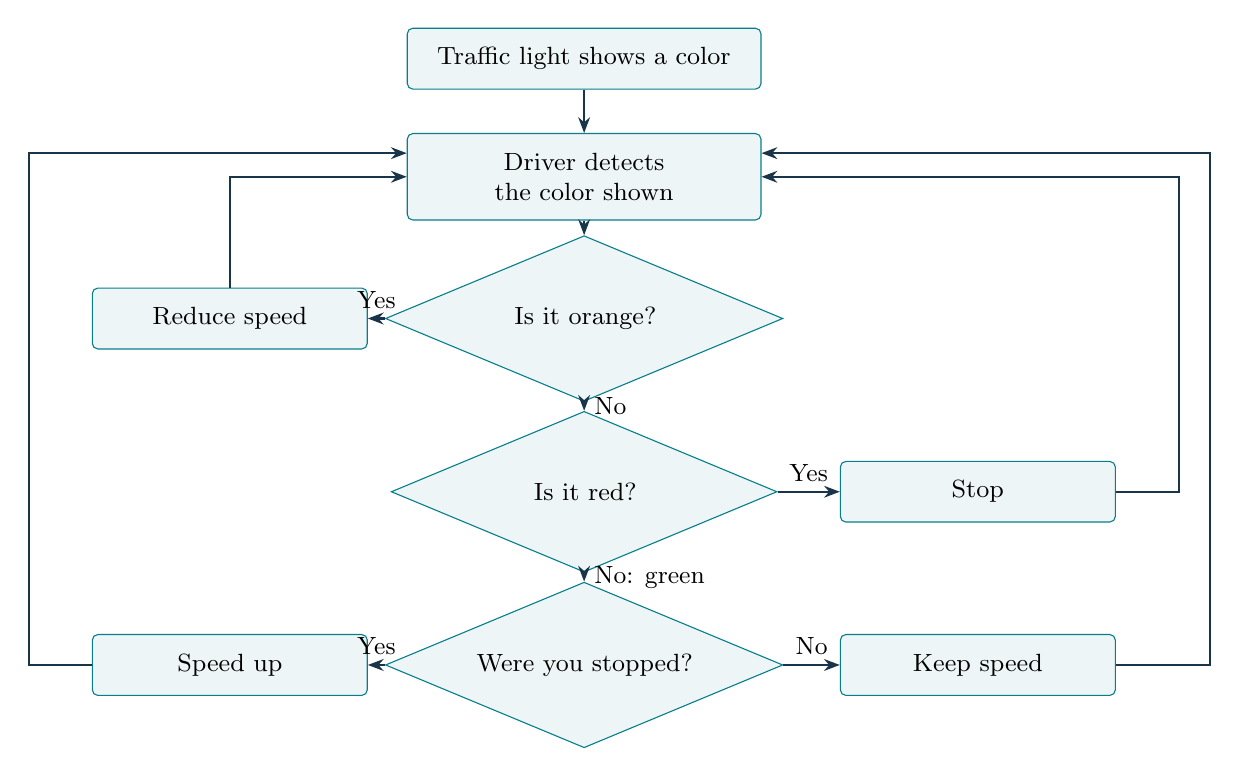
\begin{tikzpicture}
\node[box,text width=4cm] (light) at (0,0) {Traffic light shows a color};
\node[box,text width=4cm] (detect) at (0,-1.5) {Driver detects the color shown};
\node[box,diamond,rounded corners=0pt,aspect=2.4,text width=2.7cm] (orange) at (0,-3.3) {Is it orange?};
\node[box,text width=3cm] (reduce) at (-4.5,-3.3) {Reduce speed};
\node[box,diamond,rounded corners=0pt,aspect=2.4,text width=2.7cm] (red) at (0,-5.5) {Is it red?};
\node[box,text width=3cm] (stop) at (5,-5.5) {Stop};
\node[box,diamond,rounded corners=0pt,aspect=2.4,text width=2.7cm] (stopped) at (0,-7.7) {Were you stopped?};
\node[box,text width=3cm] (speedup) at (-4.5,-7.7) {Speed up};
\node[box,text width=3cm] (keep) at (5,-7.7) {Keep speed};
\draw[arr] (light)--(detect);
\draw[arr] (detect)--(orange);
\draw[arr] (orange)--node[above,font=\small]{Yes}(reduce);
\draw[arr] (reduce.north)|-(detect.west);
\draw[arr] (orange)--node[right,font=\small]{No}(red);
\draw[arr] (red)--node[above,font=\small]{Yes}(stop);
\draw[arr] (red)--node[right,font=\small]{No: green}(stopped);
\draw[arr] (stopped)--node[above,font=\small]{Yes}(speedup);
\draw[arr] (stopped)--node[above,font=\small]{No}(keep);
\draw[arr] (speedup.west)--++(.0,0)--++(-.8,0)|-([yshift=3mm]detect.west);
\draw[arr] (stop.east)--++(.8,0)|-(detect.east);
\draw[arr] (keep.east)--++(1.2,0)|-([yshift=3mm]detect.east);
\end{tikzpicture}
\end{center}
{\small\textbf{Flowchart A. Test orange first.} Orange leads to reducing speed and observing again. Otherwise, test red: stop if yes. If no, the signal is green: a stopped driver speeds up; a moving driver keeps speed. The repeated observation uses the color currently shown.}

One detection box, three decisions, and clear return paths keep the flowchart easy to follow. Returning to the same box makes repetition explicit without duplicating the operation: each visit means detecting the color again.

The stopped test reads the driver's current speed: zero means stopped. On green, speeding up gives a stopped driver a positive speed; a driver already moving retains its current speed.

Trace each color through the questions, including green for a stopped driver and for a moving driver. The \texttt{seeColor()} method updates the driver's perceived color; \texttt{adjustSpeed()} follows the appropriate response branch. On the next pass, the driver reads the color currently shown, rather than reusing the previous observation.

\subsection{Step 3: Assemble the methods into one cycle}

The return arrows mean that observation repeats on the next cycle. Execute one observation and response per driver per cycle, allowing the light to change between cycles. For this exercise, choose the following schedule:

\begin{enumerate}
\item Check whether the light's phase is due to change; call \texttt{changeColor()} when required.
\item For each driver, call \texttt{seeColor()} and then \texttt{adjustSpeed()}.
\item Record the states needed to check the cycle.
\item Advance elapsed time by one step and repeat until the stopping condition holds.
\end{enumerate}

Trace the consequence of this ordering: drivers observe the light's updated color. If observations precede the signal update, they use the previous color. Choose the order deliberately and preserve it in the implementation.


This introduces \textbf{CLOCK}: the model's organization of time and activation. Complete the cycle by answering these questions:
\begin{description}[style=nextline,leftmargin=0pt,labelindent=0pt,labelsep=0pt,labelwidth=0pt,itemindent=0pt,itemsep=4pt]
\item[Iteration and time] What does one step represent, and which operations repeat?
\item[Activation and scheduling] Which elements act during the step, and in what order?
\item[Serialization or simultaneous updates] Do elements read changes made earlier in the same step, or do all read a common starting state and store changes for later application?
\item[Synchronization] If changes are stored, when are they applied together?
\item[Termination] Does the run end after a specified number of steps, at an event, or under another explicit condition?
\end{description}

For the first exercise, use a fixed run length and a declared driver order. Later, if drivers respond to one another, test whether changing that order affects the results. Simultaneous updating requires an explicit read--calculate--apply procedure; executing agents one after another does not create it automatically.

\begin{fitdisplay}
\boxed{A_4:\ \text{HOW THINGS ARE ARRANGED}\qquad FC:\ \text{HOW THINGS HAPPEN}}
\end{fitdisplay}

If practice can change a connection, an institutional prescription, or an agent's expectations, add the corresponding update at its place in the cycle. State its conditions. Where practice maintains the existing arrangement, no forced change is needed.

\clearpage


\section{Ex Post: Writing the Model Document}

\subsection{Why document: auditability, reproducibility, and curation}

A model becomes a reusable contribution when others can understand what was built, examine its assumptions, recover its results, and continue the work. Code, diagrams, and selected plots each supply only part of that account. Documentation connects them to the question and to the model version investigated.

\begin{description}[style=nextline,leftmargin=0pt,labelindent=0pt,labelsep=0pt,labelwidth=0pt,itemindent=0pt,itemsep=5pt]
\item[Auditability] Make it possible to follow a claim through the reported results and experiments to the assumptions, processes, and implementation that produced it.
\item[Reproducibility] Record the code, inputs, settings, software environment, random-seed procedure, and analysis steps needed to recover the reported results, including the expected variation in stochastic runs.
\item[Curation] Preserve an identifiable, usable version of the work: organize the source, data provenance, run configurations, outputs, and documentation; record changes, authorship, access conditions, and instructions for future users. Curation makes later comparison, correction, and reuse possible.
\end{description}

Documentation begins during construction. Ex post, reconcile that evolving record with what was actually implemented and tested. A deliberately simple I-ABM needs this account too: parsimony reduces what must be documented, not the need to document it.

\subsection{ODD as the main documentation reference}

We adopt \textbf{ODD---Overview, Design concepts, and Details---as our main reference for model description}, using Grimm et al.'s 2020 update \cite{grimm_odd_2020}. Its seven elements are: purpose and patterns; entities, state variables and scales; process overview and scheduling; design concepts; initialization; input data; and submodels. The common structure helps readers locate, compare, and reconstruct model specifications.

ODD is especially useful for our ex-post task because it connects a specific model version to its purpose, evaluation patterns, and design rationale. The updated guidance links purpose to the study's main results and calls attention to relevant patterns the model fails to reproduce. It can also guide construction; it is not restricted to work after simulation \cite{grimm_odd_2020}.

\textbf{Distinguish the model description from the full study report.} ODD does not replace reporting computational experiments and results. Our ex-post document requires both: an ODD description of the model and an account of what its use revealed. Use ODD as the organizing reference and supplement it only where the study report requires information not already supplied there.

\subsubsection{ODD: reading the guidance and checklists}

Use this compact table alongside \emph{S1: ODD Guidance and Checklists}, the supplement to Grimm et al. (2020) \cite{grimm_odd_2020}. Retain the seven numbered elements in the model description. The eleven entries under Element 4 are design concepts, not additional numbered elements. Consult S1 for the full guidance, checklists, and examples.

\begin{center}
\begingroup\small
\renewcommand{\arraystretch}{1.15}
\begin{tabularx}{\linewidth}{@{}P{5.7cm}Y@{}}
\toprule
\textbf{ODD element or design concept} & \textbf{Information to locate or supply}\\
\midrule
\textbf{1. Purpose and patterns} & Specific purpose and patterns used to assess suitability for that purpose.\\
\textbf{2. Entities, state variables, and scales} & Represented entities, their states, and spatial and temporal scales.\\
\textbf{3. Process overview and scheduling} & Which entities do what, when, and in what order; timing of state updates.\\
\midrule
\textbf{4. Design concepts} & How the following concepts enter the model.\\
\quad Basic principles & Underlying theories, assumptions, and modeling approach.\\
\quad Emergence & Outcomes arising from interactions versus imposed behavior.\\
\quad Adaptation & How agents adjust behavior to their conditions.\\
\quad Objectives & Criteria guiding adaptive choices, where represented.\\
\quad Learning & How experience changes adaptive behavior.\\
\quad Prediction & How agents anticipate future conditions or consequences.\\
\quad Sensing & Information available to agents and how they obtain it.\\
\quad Interaction & Direct and indirect effects among entities.\\
\quad Stochasticity & Random processes and their role.\\
\quad Collectives & Groups, their formation, and their representation.\\
\quad Observation & Outputs collected and how they are recorded for analysis.\\
\midrule
\textbf{5. Initialization} & Initial entities, states, and their assignment procedures.\\
\textbf{6. Input data} & External data or drivers supplied during a run.\\
\textbf{7. Submodels} & Process rules, parameters, rationale, and results of submodel calibration, testing, and exploration.\\
\bottomrule
\end{tabularx}
\endgroup
\end{center}

The ex-post document answers:
\begin{fitdisplay}
\boxed{\begin{gathered}
\textbf{What did we build, what did we do with it,}\\
\textbf{and what can we defensibly claim from it?}
\end{gathered}}
\end{fitdisplay}

Place the LUL and flowcharts within the relevant ODD elements, and cross-reference the exploration, calibration, and tests already documented there. Where needed, supplement that account with the experiments actually conducted, their settings and replications, and the findings and limitations supporting each claim. Link the reported results to the assessed model version, saved outputs, and analysis procedures so readers can recover them without duplicating the ODD description.

\subsubsection{Version control, preregistration, and preprints}

\textbf{Version control.} Use Git to track changes to code, ODD, diagrams, and analysis scripts; GitHub is one platform for hosting and collaborating on Git repositories. Associate reported experiments with a specific commit or release, so a later revision cannot silently replace the model that produced a finding. Keep a readable change history and a README explaining how to run the model. A repository complements ODD; it does not replace the model description. See \href{https://docs.github.com/en/repositories/releasing-projects-on-github/about-releases}{GitHub's release documentation} for identifying and distributing versions.

\textbf{Preregistration.} An open-science workflow can include a dated plan deposited in a registry such as the Open Science Framework (OSF). Before the planned tests, specify the model version, questions, parameter ranges, outcomes, replication strategy, and analysis criteria. Disclose prior exploration and report deviations from the plan. Exploratory I-ABM development remains legitimate: distinguish discoveries made during exploration from subsequent tests of those discoveries. Preregistration makes that distinction visible; it does not establish model validity. See the \href{https://www.cos.io/initiatives/prereg}{Center for Open Science's preregistration guidance}.

\textbf{Preprints and accessible materials.} A preprint can circulate the model description, analyses, and findings for scrutiny before journal peer review. Identify its review status and version, link the corresponding model release and accessible supporting materials, and connect later revisions or publications to the earlier account. For professional work, agree what may be shared publicly and what requires controlled access. Openness should make the work inspectable within those conditions, without exposing confidential inputs.

\begin{principle}{Meta-analysis of simulation evidence}
In this course, \textbf{meta-analysis of simulation evidence} means assessing the model and the evidence produced across its computational experiments. It is broader than statistical meta-analysis of independent empirical studies. Name the analyses performed and report their findings; the umbrella term does not replace them. This assessment complements the ODD description rather than introducing another model-description protocol.
\end{principle}

\subsection{What P-ABM adds: documenting the professional use}

For P-ABM, the auditable model description supports a professional account of what can be done, over which horizons, and under which possible changes to the modeled world. We organize these additions around three questions. They are course guidance for professional use, rather than additional ODD elements.

\subsubsection{Policy brief: from model findings to proposed action}

ODD describes the model; it does not have the purpose or format of a policy brief. A policy brief translates the investigation into a concise account for decision-makers, ending with clear proposed actions: who can act, what they should consider doing, with which resources, and under which conditions. Connect each recommendation to the findings and their limits, while making objectives and trade-offs visible. This builds on the practical orientation to policy use discussed by Gilbert et al. \cite{gilbert_policy_2018}.

Recommendations must address the applicable legal frameworks and institutional authority. Identify the relevant jurisdictions, competencies, legislation, and coordination requirements, especially in multilevel government. Distinguish actions available under current arrangements from proposals requiring legislative or institutional change; for the latter, identify that change as a prerequisite. The model's representation of a rule does not itself establish legal authority to act.

Keep the brief accessible and link it to the technical documentation. Where strategic information is non-public, state how authorized reviewers can scrutinize the evidence. Specify responsibility for implementation, monitoring, and revising the advice. Simulation informs the decision; political judgment, negotiation, and responsibility for action remain with the decision-makers.

\subsubsection{The prospective look: recommendations across time horizons}

Our earlier discussion of Lyapunov provides a reason to examine stability and sensitivity when interpreting trajectories: small differences in starting conditions may have consequential effects over time. That possibility must be investigated for the model at hand; it does not mean that every ABM is chaotic or that one diagnostic establishes a policy forecast. Recommendations require analysis appropriate to their horizon, including sensitivity, uncertainty, and robustness across plausible conditions. Longer simulation runs alone do not establish longer-term applicability.

Define short, medium, and long term for the engagement, distinguishing the decision deadline, implementation time, and horizon of effects:
\begin{description}[style=nextline,leftmargin=0pt,labelindent=0pt,labelsep=0pt,labelwidth=0pt,itemindent=0pt,itemsep=5pt]
\item[Short term] Identify actions possible with current authority, resources, and infrastructure, their immediate constraints, and indicators for monitoring their effects.
\item[Medium term] Examine pilots, staged investments, and coordination or institutional changes. Report which findings persist across plausible assumptions and specify milestones for continuation, revision, or withdrawal.
\item[Long term] Explore alternative pathways, infrastructure, and institutions, including dependencies and changes that could invalidate present assumptions. Identify options to preserve and conditions under which the model and advice should be revisited.
\end{description}

Write prospective claims conditionally: under stated assumptions, how does an intervention alter the simulated outcomes relative to a baseline? Report the supporting experiments and uncertainty. As Polhill et al. emphasize, anticipation becomes especially demanding when future conditions include novelty beyond the current representation \cite{polhill_prediction_2021}. A useful recommendation may concern a pilot, further information gathering, or preparation for several futures, rather than a single predicted outcome.

\subsubsection{The reconfiguration of the As: social recursivity and novelty}

Practices may reproduce or transform the conditions of subsequent action. Document whether the model allows changes in agents' expectations and capabilities ($A_1$), environmental conditions ($A_2$), artifacts and institutions ($A_3$), and their arrangement ($A_4$). Explain the mechanisms, conditions, and timescales of these changes, and identify what remains fixed. This extends our situated-agency and social-recursivity discussion into the professional account \cite{knoeri}.

For example, networked infrastructure combines material Artificiality with connections and dependencies; multilevel government combines decision-making actors, institutional prescriptions, and authority relations. GIS layers may describe terrain, infrastructure, or jurisdictions, so classify their content by its modeling role. Where these structures can change, document how methods alter states or connections. Distinguish changes generated within a run from re-specifications introduced by the modeler between scenarios. Invented $A_3$ can open useful possibilities, but its assumed capabilities and requirements must remain explicit.

Here we place \textbf{Axelrod's parsimony and Polhill et al.'s concerns about novelty in productive tension}, as a course comparison rather than a direct dispute between the authors. Axelrod's advice helps us construct understandable models that develop and test intuition \cite{axelrod_complexity_1997}. Polhill et al. ask what happens when relevant future entities, processes, or categories exceed a model's possibilities \cite{polhill_prediction_2021}. A model can change states and connections while still being unable to generate a new kind of institution or action. Document that boundary and assess its importance for the proposed use. We can retain a parsimonious model while making clear which reconfigurations it investigates and which require a new specification.

\begin{principle}{A developing professional frontier}
The more ambitious forms of P-ABM can depend heavily on advanced mathematical analysis, programming, and computational resources, particularly when investigating many interacting mechanisms and possible futures. Their development expands the scope of what we can attempt; computational limits today need not define the field's eventual possibilities. Faster computation nevertheless does not by itself resolve missing knowledge or justify a recommendation.

For present practice, Axelrod's advice remains a strong foundation: start with an effective abstraction, preserve interpretability, and investigate what the model can teach us. Our ambition extends further as methods and computational capabilities advance. P-ABM can contribute useful work now while opening a path toward more demanding forms of anticipation and decision support.
\end{principle}

\clearpage
\section*{References and source boundaries}
\addcontentsline{toc}{section}{References and source boundaries}
The entries below document the works explicitly cited in this guide, including the earlier readings named in the opening and the foundations summarized in Section~\ref{sec:previous-foundations}. This bibliography is not the roster of the six new readings for this session, nor a complete bibliography of prior course readings. Giddens and Ostrom are discussed through Knoeri et al. and Ghorbani et al.; Lakatos is discussed through Cioffi-Revilla. This document does not claim independent consultation of their original books. Axelrod supports the discussion of simplicity and intuition; Gilbert et al. ground the discussion of professional policy-modeling practice, collaboration, abstraction, and use; Polhill et al. support the discussion of computational limits, novelty, and the scope of prospective claims. The professional framing through the Four As, invented Artificiality, and the lunar illustration are course synthesis.

\begingroup\small
\begin{thebibliography}{99}
\bibitem{weaver} Weaver, W. (1948). Science and complexity. \emph{American Scientist}, 36(4), 536--544.
\bibitem{simon} Simon, H. A. (1962). The architecture of complexity. \emph{Proceedings of the American Philosophical Society}, 106(6), 467--482.
\bibitem{epstein} Epstein, J. M. (1999). Agent-based computational models and generative social science. \emph{Complexity}, 4(5), 41--60.
\bibitem{cioffi} Cioffi-Revilla, C. (2010). A methodology for complex social simulations. \emph{Journal of Artificial Societies and Social Simulation}, 13(1), 7. \url{https://jasss.soc.surrey.ac.uk/13/1/7.html}
\bibitem{knoeri} Knoeri, C., Binder, C. R., \& Althaus, H.-J. (2011). An agent operationalization approach for context specific agent-based modeling. \emph{Journal of Artificial Societies and Social Simulation}, 14(2), 4. \url{https://jasss.soc.surrey.ac.uk/14/2/4.html}
\bibitem{ghorbani} Ghorbani, A., Bots, P., Dignum, V., \& Dijkema, G. (2013). MAIA: A framework for developing agent-based social simulations. \emph{Journal of Artificial Societies and Social Simulation}, 16(2), 9. \url{https://jasss.soc.surrey.ac.uk/16/2/9.html}

\bibitem{simon_behavioral_1955} Simon, H. A. (1955). A behavioral model of rational choice. \emph{The Quarterly Journal of Economics}, 69(1). \url{https://doi.org/10.2307/1884852}.
\bibitem{axtell_why_2000-1} Axtell, R. (2000). \emph{Why agents? On the varied motivations for agent computing in the social sciences}. Working Paper No.~17. Washington, D.C.: The Brookings Institution.
\bibitem{macy_factors_2002} Macy, M. W., \& Willer, R. (2002). From factors to actors: Computational sociology and agent-based modeling. \emph{Annual Review of Sociology}, 28(1), 143--166. \url{https://doi.org/10.1146/annurev.soc.28.110601.141117}.
\bibitem{kollman_chapter_2006} Kollman, K., \& Page, S. E. (2006). Computational methods and models of politics. In \emph{Handbook of Computational Economics}, Vol.~2, Chapter~29, pp.~1433--1463. Elsevier. \url{https://doi.org/10.1016/S1574-0021(05)02029-0}.

\bibitem{axelrod_complexity_1997} Axelrod, R. M. (1997). \emph{The complexity of cooperation: Agent-based models of competition and collaboration}. Princeton, NJ: Princeton University Press. \url{https://doi.org/10.1515/9781400822300}.
\bibitem{axelrod_dissemination_1997} Axelrod, R. (1997). The dissemination of culture: A model with local convergence and global polarization. \emph{Journal of Conflict Resolution}, 41(2), 203--226. \url{https://doi.org/10.1177/0022002797041002001}.
\bibitem{grimm_odd_2020} Grimm, V., et al. (2020). The ODD protocol for describing agent-based and other simulation models: A second update to improve clarity, replication, and structural realism. \emph{Journal of Artificial Societies and Social Simulation}, 23(2), 7. \url{https://doi.org/10.18564/jasss.4259}
\bibitem{gilbert_policy_2018} Gilbert, N., Ahrweiler, P., Barbrook-Johnson, P., Narasimhan, K. P., \& Wilkinson, H. (2018). Computational modelling of public policy: Reflections on practice. \emph{Journal of Artificial Societies and Social Simulation}, 21(1), 14. \url{https://doi.org/10.18564/jasss.3669}
\bibitem{polhill_prediction_2021} Polhill, J. G., Hare, M., Bauermann, T., Anzola, D., Palmer, E., Salt, D., \& Antosz, P. (2021). Using agent-based models for prediction in complex and wicked systems. \emph{Journal of Artificial Societies and Social Simulation}, 24(3), 2. \url{https://doi.org/10.18564/jasss.4597}
\end{thebibliography}
\endgroup

\begin{principle}{How to read the attributions}
\raggedright
\textbf{Reading-grounded:} organized complexity; hierarchical organization and near-decomposability; generative explanation and its limits; progressive model sequences; context-specific situated agency; institutional action and possible non-compliance; Axelrod's emphasis on simplicity and on simulation as an aid to intuition; professional policy-modeling practice and collaboration; computational limits and the evidential challenges of endogenous novelty.

\textbf{Course synthesis:} bottom-up + along the way; the history statement and Simon/Giddens bridge; Four As, six relational classes, situated-agency triad, and dynamic practice notation; the parsimonious I-ABM heuristic and the distinction between $A_{3m}$ and $A_{3s}$; progressive re-specification; restricted LUL; auditability and actionability; broad meta-analysis of simulation evidence; prospective claims; and the traffic and lunar teaching illustrations.
\end{principle}
\end{document}
